\documentclass{article}
\usepackage{microtype}
\usepackage{graphicx}
\usepackage{subfigure}
\usepackage{booktabs}
\usepackage{hyperref}
\newcommand{\theHalgorithm}{\arabic{algorithm}}
\usepackage[accepted]{icml2018}
\icmltitlerunning{Russian Raions Data Exploration}

\begin{document}

\twocolumn[
\icmltitle{Russian Raions Data Exploration: \\
           The Final Project of Applied Multivariate Statistics}
\begin{icmlauthorlist}
\icmlauthor{Li Ziyao, 1500017776}{}
\end{icmlauthorlist}
\icmlkeywords{Russian Raions, Data Exploration, Applied Multivariate Statistics}
\vskip 0.3in
]

\begin{abstract}
In this project, data of 125 Russian raions is explored in attempt to find some connections between the average house prices and some other basic features of the raions. Several methods of multivariate statistic analysis, including Principal Components Analysis, Factor Analysis and linear regression, are implemented. The results show that the predictors in the given data cannot adequately explain the variance of the house price, but important predictors, such as industrial area proportions, can be somehow instructive.
\end{abstract}

\section{Introduction}

House prices can depend on different variables, among which location is considered the most important. House prices among different areas are usually different. In this project, average house price data, along with some basic descriptions of over a hundred Russian raions are analysed in order to seek some connections between the house price and the location.

Different methods of multivariate statistic analysis are implemented in this project, including Principal Component Analysis(PCA), Factor Analysis, Linear Regression, etc. Different methods provide different perspectives of the data and show consistent results.

\section{Data Description}

\subsection{Data Source}

The original data is from a relevant Kaggle competition\footnote
{https://www.kaggle.com/c/sberbank-russian-housing-market}. The goal of the competition is to predict accurate prices of individual properties transacted during 2013 and 2016 in Russia. Hundreds of attributes of the properties are given, including detailed information of the raions of the properties. The data is large but somehow dirty due to obvious inconsistencies and a considerable percentage of missing data. For accuracy and simplicity, only the extracted data of different Russian raions are implemented in this project. The attributes of the data are:

\begin{itemize}
\item \textbf{Raion Name:} the name of the raion.
\item \textbf{Area:} the total area of the raion.
\item \textbf{Population:} the total population of the raion.
\item \textbf{Population Age Structure:} including the population of people younger than working age, during working age and elder than working age.
\item \textbf{Ground Usage:} the proportions of area of ​​greenery and of industrial zones of ​​the total area.
\item \textbf{Raion Facilities:} including the numbers of healthcare centers, the number of top-20 Universities across Russia in the raion; and whether thermal power plants, incinerations, dirty industries (implemented as "oil chemistry"), radioactive waste disposals, railroad terminals, big markets and nuclear reactors are in the raion.
\end{itemize}

\subsection{Data Preprocessing}

Although the data itself is elaborately selected, necessary preprocessing is still in need. The preprocessing includes:

\begin{itemize}
\item \textbf{Dealing with Missing Data:} Several attributes and samples suffering severely from missing data are abandoned. A few missing data are filled with 0, according to the context.
\item \textbf{Reduce Collinearity:} Obvious collinearity is removed, such as the attribute "work population", since the sum of three kinds of population always equals to the total population of the raion.
\item \textbf{Other Implementations:} The real amounts of three kinds of populations are replaced with their proportions. Yes/No data are replaced with 1/0.
\end{itemize}

The final data determined in this project contains 125 samples, and 17 attributes of each sample.

\section{Data Explorations}

Firstly, a pairwise scatter plot is drawn to identify extreme outliers\footnote{Results are shown in the appendix.}. 4 samples are identified as outliers. A histogram is drawn for each numerical attribute to test for normality, and the results are shown in Figure~\ref{fig1}.

\begin{figure}[ht]
\vskip 0.2in
\begin{center}
\centerline{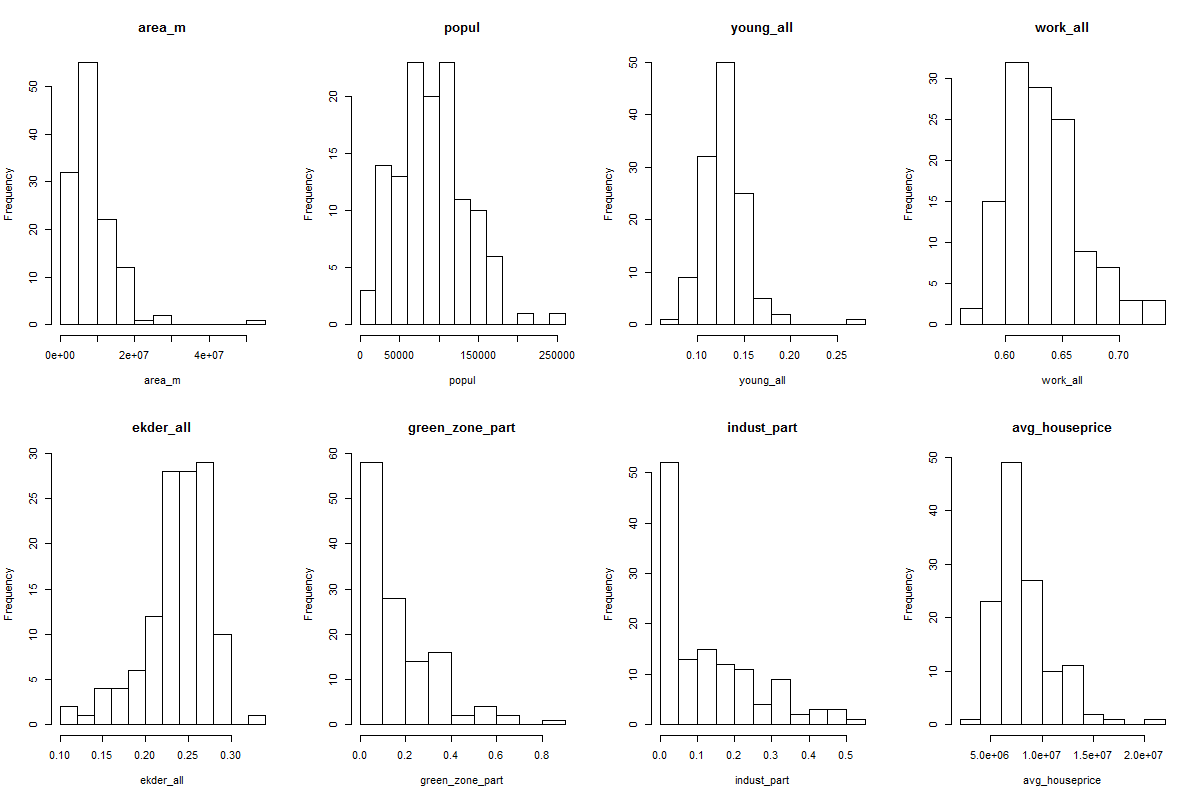
\includegraphics[width=\columnwidth]{numer_hists}}
\caption{Histograms of numerical variables before transformations.}
\label{fig1}
\end{center}
\vskip -0.2in
\end{figure}

\begin{figure}[ht]
\vskip 0.2in
\begin{center}
\centerline{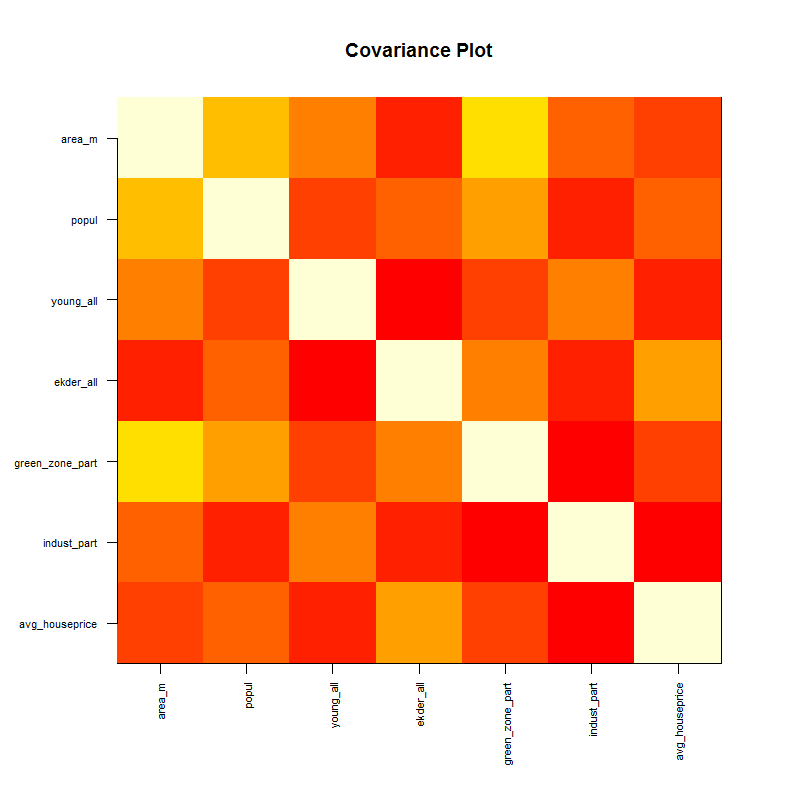
\includegraphics[width=\columnwidth]{cov_plot}}
\caption{Correlation of numerical variables. The brighter the grid is, the larger the covariance is.}
\label{fig2}
\end{center}
\vskip -0.2in
\end{figure}

From Figure~\ref{fig1}, most variables do not seem to be normally distributed. Necessary transformations are implemented to satisfy the normality assumption: a Box-Cox transformation with an estimated $\lambda$ is applied on area, population and price variables; a logit transformation is applied on all proportional variables, which is a typical transformation for such variables\footnote{The original proportions are all added with 1\% to correctly handle 0s.}. After such transformations, the normality assumption is tested accepted by a chi-square plot\footnote{Results are shown in the appendix.}.

Although all categorical are binary and are easily replaced with 0/1 dummy variables, it is usually hard to include them into a multivariate normal distribution. Similar situations are happening on some count variables of the model, but is not a serious problem due to the small numbers of kinds of values of these variables.

Figure~\ref{fig2} is a correlation plot of the numerical variables, from which we can see a high correlation between raion area and the percentage of greeneries, and one between raion area and raion populations; negative correlations can be observed between industrial area and green-zone area proportions, and between young and old population proportions. Some negative correlations can be observed between house price and other variables, but few of them are significant.

\section{Principal Components \& Factor Analysis}

\subsection{Principal Components Analysis}

\label{PCA}

\begin{figure}[ht]
\vskip 0.2in
\begin{center}
\centerline{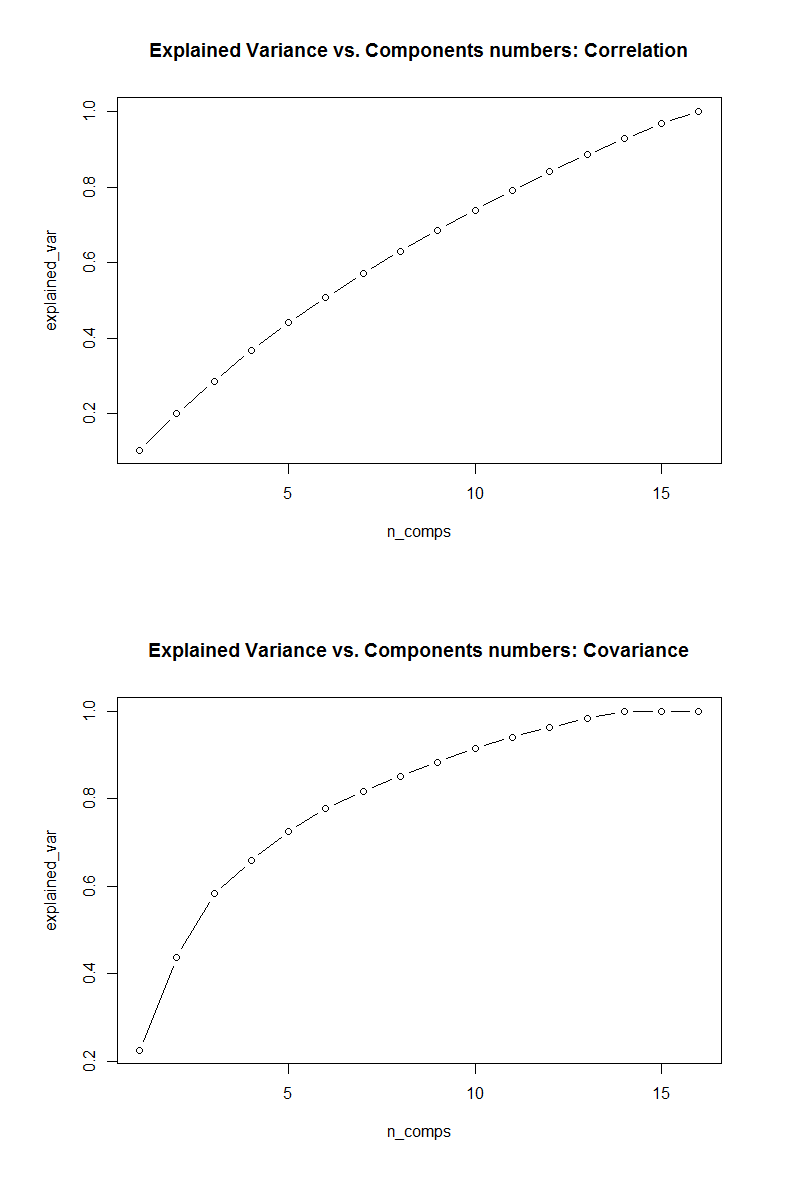
\includegraphics[width=\columnwidth]{pca_graph_cor_cov}}
\caption{Principal components graphs. The graph shows the proportion of total explained variance versus the number of the components. The first graph is almost linear, which suggest that the data is hardly compactable, i.e. any attempt to reduce the data dimension can lead to a considerable loss of information; the second graph shows that the data is easier to compress.}
\label{fig3}
\end{center}
\vskip -0.2in
\end{figure}

In order to reduce dimensions, a Principal Component Analysis (PCA) is implemented on both the total data and the numerical data. Results are similar, and here the results of total data is chosen to demonstrate.

Figure~\ref{fig3} shows the corresponding variation of total proportion of explained variance when increasing the number of components, under both correlation matrix and covariance matrix.

It is interesting to see the huge difference between two methods. When implementing PCA with the correlation matrix, the function is nearly linear, which suggests that the data is hard to compress, or any attempt to reduce the data dimension may lead to a considerable loss of information, and no dominant component emerges; while implemented with the covariance matrix, the data becomes much easier to compress, and the first three components explained nearly 60\% of total variance. This happens probably because of the great variety of variance of different variables in the data, i.e. the diagonal elements of the covariance matrix varies greatly, while all diagonal elements of the correlation matrix is 1.

\subsection{Factor Analysis}

As the results of PCA shows, the data is somehow hard to compress. Therefore, it is hard to attribute the hold variability to a few factors. However, applying a factor analysis is still instructive when choosing an appropriate number of factors.

After several attempts, a factor model with five factors is implemented. The variance proportion explained by this factor model is 43\%. According to the detailed results shown in Table~\ref{tab1}, the five factors can be named as "General Size", "Public Facilities", "Vigor", "Industries", "Oil Chemistries" according to their significant loadings of different variables.

\label{FA}

As for the average house price, from the results above, is positively correlated with "Public Facilities" and negatively correlated with "Vigor" and "Industries". Raions with better public facilities usually have higher house prices, and industrial raions have lower house prices. With more population under work age, the raions also have lower house prices.

\begin{table}[t]
\caption{Factor loadings of different variables.}
\label{tab1}
\vskip 0.15in
\begin{center}
\begin{small}
\begin{sc}
\begin{tabular}{lrrrrr}
\toprule
Variables & F1 & F2 & F3 & F4 & F5  \\
\midrule
area & .891 &  & .355 & .138 & \\
popul & .494 &  &  &  & \\
young & -.101 &  & .659 & -.177 & \\
ekder &  &  & -.586 &  & \\
green\_part & .585 & -.374 & -.180 & -.326 & \\
indust\_part & -.238 & -.175 & .332 & .821 & \\
healthcare & .261 & .317 & -.129 & .234 & \\
univ\_top\_20 &  & .699 &  & -.166 & \\
thermal & .139 &  &  & .353 & .154\\
incin &  &  & .427 &  & \\
oil\_chem &  &  &  & .151 & .984\\
radio & .339 & .157 &  & .124 & \\
rail &  & .541 &  &  & \\
market &  &  &  &  & .282\\
nuclear &  &  & -.129 & .317 & \\
houseprice &  & .556 & -.326 & -.200 & -.154\\
\bottomrule
\end{tabular}
\end{sc}
\end{small}
\end{center}
\vskip -0.1in
\end{table}

\section{Least Square Regression}
In this section, an Ordinary Least Square (OLS) is implemented on the full data, with the house price being the target variable and others being predictors.

Firstly, two different methods are tested. The first one regress the original house price on the predictors, and the second one regress the Box-Cox-transformed house price variable on the same predictors. Despite a better approximation to a normal distribution, the Box-Cox regression behaves much poorly than the ordinary regression, with correspondent R-squares 0.39 and 0.47. In the latter model, proportions of industrial area seem to be the most important predictor of the raions' house prices. The higher the proportions are, the lower the prices are. This agrees with the results obtained from the Factor Model in Section~\ref{FA}. Other variables are less dominant\footnote{Detailed results are in the appendix.}.

From the reported R-square, the regression model is not adequate, and the residual plot supports this conclusion, see Figure~\ref{fig4}. Clear linear trend can be seen in the plot, suggesting that the predictors cannot adequately explain the variability of the house price.

Sometimes, a model can be inadequate due to regardlessness to the interactions between different categorical variables. A fully interactive model, i.e. all possible interactive categories are one-hot labeled, is established to exclude this probability. The R-square of the fully interactive model is 0.50. Considering the great many variables added into the model, the improvement is far from significant, and the model is still inadequate. Therefore, there is no significant interactive effect of the categorical models in the regression.

\begin{figure}[ht]
\vskip 0.2in
\begin{center}
\centerline{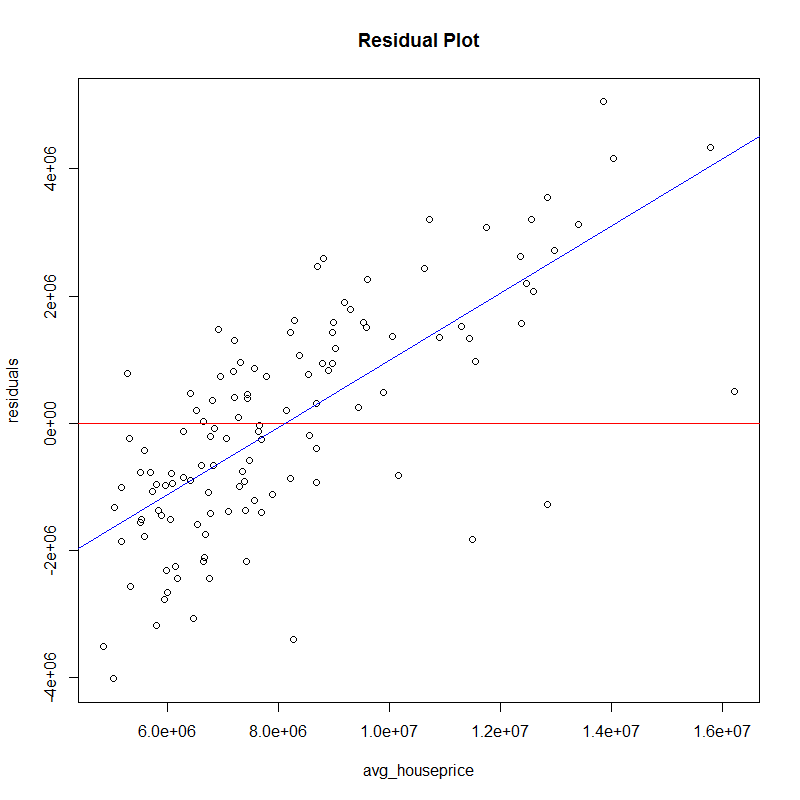
\includegraphics[width=\columnwidth]{residual_y_plot}}
\caption{Residual plot of the OLS regression. The horizontal axis is the house prices, and the vertical axis is the residuals.}
\label{fig4}
\end{center}
\vskip -0.2in
\end{figure}

\section{Comparison Between \\ Different Regression Models}

In this section, different linear regression models are compared on this task.

The data is split into training data (80\%) and test data (20\%). Five different linear regression models are implemented, including simple OLS, stepwise OLS, two models with regularization - LASSO and ridge regression, and Principal Components Regression (PCR). The results are estimated with Root Mean Square Error (RMSE) and shown in Table~\ref{tab2}.

\begin{table}[t]
\caption{Different linear models' performances on the test set, with regard to Root Mean Square Error (RMSE).}
\label{tab2}
\vskip 0.15in
\begin{center}
\begin{small}
\begin{sc}
\begin{tabular}{lr}
\toprule
Methods & RMSE \\
\midrule
OLS & $2.178 \times 10^6$ \\
stepwise OLS & $2.347 \times 10^6$ \\
Ridge & \textbf{$2.073 \times 10^6$} \\
LASSO & $2.154 \times 10^6$ \\
PCR(K=10) & $2.092 \times 10^6$ \\
\bottomrule
\end{tabular}
\end{sc}
\end{small}
\end{center}
\vskip -0.1in
\end{table}

Two regularization methods out-performed the simple OLS, since most of the predictors contribute little to the target variable; however, the stepwise OLS performs poorly. This could be a consequence of the incompressibility mentioned in Section~\ref{PCA}. Simply omitting variables according to AIC leads to a decline of performance on the test set. The performance of PCR is also good, since the total proportion of variance loss with K=10 is only 8.50\%. However, none of these models are adequate according to residuals analysis, and this is decided by the quality of data predictors. More complicated models can be introduced to alleviate this problem, such as Gradient Boosting and Neural Network.

\section{Conclusion}
In previous sections, different methods of multivariate statistic analysis are implemented in attempt to obtain the relation between the house price and some basic features of Russian raions. Among all the predictors given in the dataset, the proportion of industrial area is the dominant variable. This may suggest that how much life is bothered by industries is an crucial factor of house price, or some more complicated mechanisms lead to this phenomenon. Further experiments and analysis is required to have a more specific conclusion.

Although machine learning techniques do provide better predictions on the house price, they are usually less or even not at all interpretable. On the contrast, statistic models are more about predicting "rightly" than predicting more accurately. The better interpretability is the biggest advantage of statistic models.

\nocite{AMSA}
\nocite{MASS}
\nocite{forecast1}
\nocite{forecast2}

\bibliography{bib}
\bibliographystyle{icml2018}

\appendix
Codes and detailed graphs and summaries are submitted in codes.r, codes.md, codes.pdf and other sources.

\end{document}
